\documentclass{report}
\usepackage{settings}  % подклчючение настроек документа


\begin{document}

%%%% Вставка необходимого титульника %%%%
%\thispagestyle{titlepage} % Для размещения Иркутск в нижнем колонтитуле
%\newpage
    \begin{center}
    \linespread{1}
		Министерство науки и высшего образования  Российской Федерации\\
федеральное государственное бюджетное образовательное учреждение\\
высшего образования\\
«Иркутский государственный университет»\\
(ФГБОУ ВО «ИГУ»)\\
Факультет бизнес-коммуникаций и информатики 
    \end{center}
\vspace{1cm}    
\hspace{8cm} 
\begin{minipage}{0.5\textwidth}
\linespread{1}

  \begin{flushleft}
	\small{
    Кафедра естественнонаучных дисциплин \\%\vspace{-2cm}
Допускается к защите \\
и.о. зав. кафедрой, к.ф.-м.н., доцент \\
\rule{2,1cm}{0,1pt} А.Г. Балахчи\\		
            «\rule{0,9cm}{0,1pt}»\rule{2,7cm}{0,1pt} 202\,\rule{0,2cm}{0,1pt} г \\		}
		%\vspace{2еm}
		
		
		%\vspace{4.0em}
		\end{flushleft}
\end{minipage}


    \vspace{2cm} %вертикальное расстояние
    \begin{center}
   {\bf ВЫПУСКНАЯ КВАЛИФИКАЦИОННАЯ РАБОТА БАКАЛАВРА ИЛИ КУРСОВАЯ РАБОТА\\
    по направлению  \\
		09.03.03 Прикладная информатика\\
		%\vspace{1em}
		профиль\\
		«Название профиля»\\}
    \end{center}
		
		%\vspace{2.5em}%вертикальное расстояние
    \begin{center}
  		Название выпускной квалификационной работы или курсовой работы\\
    \end{center}
		
		\vspace{2.5em}
		
   \hspace{-5em} 


\noindent
\begin{minipage}[t]{0.5\textwidth}
  \begin{flushleft}
  \linespread{1}
	\small{
    Консультант: должность, ученое звание \\
  Место работы\\
        \rule{1,8cm}{0,1pt} ФИО (в именительном падеже)\\
	\vspace{2em}
		
	Нормоконтролёр: должность, уч. зв,\\
            \rule{1,8cm}{0,1pt} ФИО (в им. падеже)\\
}
		%\vspace{2em}
		
		
		%\vspace{4.0em}
		\end{flushleft}
\end{minipage}%\hspace{1em} 
\begin{minipage}[t]{0.5\textwidth}
  \begin{flushleft}
  \linespread{1}
	\small{
    Студент ** курса
	** формы обучения \\
  группа **\\
        \rule{1,8cm}{0,1pt} ФИО (в им. падеже)\\
	\vspace{2em}
		
	Руководитель: уч. степень, уч. звание\\
            \rule{1,8cm}{0,1pt} ФИО (в им. падеже)\\
\vspace{2em}
 Работа защищена:\\
        «\rule{0,9cm}{0,1pt}»\rule{2,7cm}{0,1pt} 202\,\rule{0,2cm}{0,1pt} г \\
с оценкой \rule{1,8cm}{0,1pt}\\
Протокол № \rule{0,9cm}{0,1pt}}
		%\vspace{2em}
		
		
		%\vspace{4.0em}
		\end{flushleft}
\end{minipage}
\vfill

% Изменить год в надписи <<Иркутск 202*>> нужно в файле settings.sty на 221 строке

\newpage  % Титульный лист дипломной работы 
\thispagestyle{titlepage}
%\newpage

    \begin{center}
    \linespread{1}
		Министерство науки и высшего образования  Российской Федерации\\
федеральное государственное бюджетное образовательное учреждение\\
высшего образования\\
«Иркутский государственный университет»\\
(ФГБОУ ВО «ИГУ»)\\
Факультет бизнес-коммуникаций и информатики 
    \end{center}
\vspace{1cm}    
\hspace{8cm} 
\begin{minipage}{0.5\textwidth}
\linespread{1}
%подписи для ВКР в курсовой можно удалить или заменить на настройку вертикального расстояния
  \begin{flushleft}
	\small{
    Кафедра естественнонаучных дисциплин \\%\vspace{-2cm}
Допускается к защите \\
и.о. зав. кафедрой, к.ф.-м.н., доцент \\
\rule{2,1cm}{0,1pt} А.Г. Балахчи\\		
            «\rule{0,9cm}{0,1pt}»\rule{2,7cm}{0,1pt} 202\,\rule{0,2cm}{0,1pt} г \\		}
		%\vspace{2еm}
		
		
		%\vspace{4.0em}
		\end{flushleft}
\end{minipage}


    \vspace{2cm} %вертикальное расстояние
    \begin{center}
   {\bf ВЫПУСКНАЯ КВАЛИФИКАЦИОННАЯ РАБОТА БАКАЛАВРА ИЛИ КУРСОВАЯ РАБОТА\\
    по направлению  \\
		09.03.03 Прикладная информатика\\
		%\vspace{1em}
		профиль\\
		«Название профиля»\\}
    \end{center}
		
		%\vspace{2.5em}%вертикальное расстояние
    \begin{center}
  		Название выпускной квалификационной работы или курсовой работы\\
    \end{center}
		
		\vspace{2.5em}
		
   \hspace{-5em} 


\noindent
\begin{minipage}[t]{0.5\textwidth}
  \begin{flushleft}
  \linespread{1}

		%\vspace{2em}
		
		
		%\vspace{4.0em}
		\end{flushleft}
\end{minipage}%\hspace{1em} 
\begin{minipage}[t]{0.5\textwidth}
  \begin{flushleft}
  \linespread{1}
	\small{
    Студент ** курса
	** формы обучения \\
  группа **\\
        \rule{1,8cm}{0,1pt} ФИО (в им. падеже)\\
	\vspace{2em}
		
	Руководитель: уч. степень, уч. звание\\
            \rule{1,8cm}{0,1pt} ФИО (в им. падеже)\\
\vspace{2em}
 Работа защищена:\\
        «\rule{0,9cm}{0,1pt}»\rule{2,7cm}{0,1pt} 202\,\rule{0,2cm}{0,1pt} г \\
с оценкой \rule{1,8cm}{0,1pt}\\
Протокол № \rule{0,9cm}{0,1pt}}
		%\vspace{2em}
		
		
		%\vspace{4.0em}
		\end{flushleft}
\end{minipage}

    \vfill
% Изменить год в надписи <<Иркутск 202*>> нужно в файле settings.sty на 221 строке
    
\newpage  % Титульный лист курсовой работы
%
\includepdf[pages={1}]{TitlePages/title2024.pdf} % Ваш титульний лист в .pdf 

%(если ваш титульный лист в формате .docx - воспользуйтесь сервисом по конвертации из docx (Word) в pdf)


\setcounter{page}{2} % начинаем нумерацию страниц
\tableofcontents  % это содержание, которое генерируется автоматически

\setcounter{chapter}{0} % установка счетчика глав
\setcounter{section}{0} % установка счетчика разделов
\setcounter{subsection}{0} % установка счетчика подразделов
\setcounter{equation}{0} % установка счетчика формул


\chapter*{ВВЕДЕНИЕ} % звездочка нужна, чтобы не было нумерации у этой главы
\addcontentsline{toc}{chapter}{ВВЕДЕНИЕ} % чтобы глава отображалась в содержании

Во введении указывается {\bf актуальность} и новизна темы, прописываются цель курсовой/дипломной и задачи, которые нужно выполнить для ее достижения. Не стоит указывать те цели, которые не были достигнуты. Дипломные и курсовые работы оцениваются в основном по соответствию целям и задачам, которые были прописаны во введении. Задачи указываются списком. Всё, что выделено жирным в этой главе, должно быть выделено жирным и в Вашей работе тоже. Использовать жирное начертание в других частях Вашей работы запрещено требованиями.

{\bf Объект исследования:}  формулировка объекта исследования, определяемого актуальностью. Какая область (сфера) темы исследования?

{\bf Предмет исследования:} формулировка объекта исследования, как уточнение и сужение объекта. Что конкретно изучается в выбранной области исследования?

{\bf Цель исследования:} формулировка цели работы. Какой конечный результат исследования? На что направлено исследование?

{\bf Задачи:}
\begin{enumarabic}
\item задача 1;
\item задача 2;
\item задача 3.
\end{enumarabic}


{\bf Теоретическая новизна исследования (если есть)} заключается в том, что ... (новина может быть связана со старыми идеями и выражается в их углублении, дополнении, а может быть связана с новыми идеями, выдвигаемыми лично исследователем. Отвечает на вопрос: какой вклад сделал автор в исследование проблемы?)

{\bf Практическая значимость исследования (если есть)} заключается в том, что ... (описание того, как могут применяться результаты работы, какую пользу она принесет. Отвечает на вопрос: Ради чего делалась эта работа?)

% 
\setcounter{section}{0} % обнуление счетчика разделов перед новой главой
\setcounter{subsection}{0} % обнуление счетчика подразделов перед новой главой
\setcounter{equation}{0} % обнуление счетчика формул перед новой главой

\chapter{НАЗВАНИЕ ПЕРВОЙ ГЛАВЫ КУРСОВОЙ ИЛИ ВЫПУСКНОЙ КВАЛИФИКАЦИОННОЙ РАБОТЫ}

\section{Название первого параграфа первой главы выпускной работы}

Первая глава чаще носит теоретический характер. Прописываются инструменты, которые используются в работе, обсуждается сравнение нескольких инструментов и обосновывается, почему был сделан выбор в пользу определенных инструментов. Делается анализ литературы по теме курсовой работы: кто еще делал подобные исследования и какие были результаты, как вообще проводятся исследования задач, подобных задачам в курсовой, какие подходы существуют, и почему был выбран именно такой подход.

\section{Общие нюансы оформления работы с использованием шаблона \LaTeX}
Курсовая или дипломная работа оформляется по требованиям ИГУ основанных на ГОСТ 7.32---2001 с некоторыми изменениями. То, что там не прописано, можно брать из более свежего ГОСТ 7.32---2017 <<Отчёт о научно-исследовательской работе>>. Шаблон оформлен в соответствии с этими требованиями ИГУ и ГОСТ 7.32---2017. 

Важные советы будут прописаны как в тексте шаблона, так и в комментариях к коду. Более подробная информация находится в методических материалах к этому шаблону.

Список использованных источников должен быть выполнен в соответствии с ГОСТ Р ГОСТ 7.1—--2003 <<Библиографическая запись. Библиографическое описание. Общие требования и правила составления>>. Несколько примеров оформления источников будут представлены в соответствующей главе.

Максимальная вложенность подглав в курсовой или дипломной работе --- \break 2 уровень. То есть, подглавы 1.1.1 в курсовой работе быть не может. Если необходим такой уровень, то пишется название на новой строке с красной строки без точки на конце, выделять жирным не нужно. Пример ниже.

Пример заголовка третьего уровня

Если вы описываете своими словами или напрямую цитируете текст другой работы, то нужно указать такую метку \cite{bib_gost1}. В тексте работы должны находиться ссылки на все источники из списка использованных источников. Если вы хотите сослаться сразу на несколько работ, то метка выглядит так \cite{bib_gost2}---\cite{bib_electr_res}. Источники в списке должны идти в том порядке, в котором они упоминаются в тексте. Проверяйте, что ссылки сработали правильно, и там не стоят знаки вопроса [?].

Следите за использованием тире (---) и дефисов (-). Дефис — орфографический знак, разделяющий части слова (всё-таки, во-первых), короткий, без пробелов.
Тире — пунктуационный знак, ставится между словами, длинное, отделяется пробелами с обеих сторон. Пример использования тире: Грамоте учиться — всегда пригодится. Пример использования дефиса: Разрабатывая веб-приложение, программист сталкивается с необходимостью оптимизации базы данных.

Обращайте внимание на переносы строк в тексте вашей работы. Бывает, что получаются <<висячие строки>> (когда меньше 3 букв на строке), которых не должно быть в работе. Пример изображен на рисунке \ref{fig:pic11}. В таких ситуациях следует вручную указать перенос строки с помощью \verb|\break|. Так же помните про правила переноса тире.

% Классический способ вставки рисунка
% \vspace{3mm}
% \begin{figure}[h]
% \centering
%     
\includegraphics[width=0.9\linewidth]{vis_str.png}
%     \captionsetup{justification=centering, format=plain}
%     \caption{Висячая строка}
%     \label{fig:pic11}
% \end{figure}

% Краткий способ вставки рисунка
\myfigure{0.9}{vis_str.png}{Висячая строка}{pic11}

Не допускайте разделения на две страницы названия раздела и текста раздела, списка, рисунка и подписи к рисунку, таблицы и подписи к таблице. В таких случаях можно использовать тот же \verb|\break|, комбинацию команд \verb|\hfill\break| для смещения на одну строку или команду \verb|\newpage|, которая переносит последующий текст на следующую страницу.


Крайне важно следить за орфографией и пунктуацией текста вашей работы. \LaTeX\ будет контролировать правописание, если в левом верхнем углу в Menu(Меню) --> Spell check (Проверка орфографии) поставить русский язык, но намного удобнее воспользоваться сторонним инструментом. Для проверки орфографии, пунктуации и стилистики вашего текста существует расширение для браузера Chrome под названием LanguageTool (https://languagetool.org/ru/overleaf), которое совместимо с Overleaf. Кроме того, данное расширение предлагает и другие полезные функции для работы с текстом.

\section*{Выводы по главе}
\addcontentsline{toc}{section}{Выводы по главе}
В данной главе было рассмотрено ... (Краткое обобщенное описание того, что было в главе).


\chapter{НАЗВАНИЕ ВТОРОЙ ГЛАВЫ КУРСОВОЙ ИЛИ ВЫПУСКНОЙ КВАЛИФИКАЦИОННОЙ РАБОТЫ}
% снова обнуляем счетчики section, subsection и equation в новой главе
\setcounter{section}{0}
\setcounter{subsection}{0}
\setcounter{equation}{0}
\section{Название первого параграфа второй главы}

Вторая глава носит практическую направленность. В ней нужно описать процесс работы над темой. Подробно расскажите о том, как реализовано и устроено то, что вы сделали. Активно используйте небольшие рисунки, таблицы, формулы, листинги кода. 

\section{Оформление различных элементов}

Важно проследить за оформлением списков (перечислений) в своей работе. Перечисления бывают простые и сложные, маркированные и нумерованные. Перечисления отделяются точкой с запятой. В конце перечисления всегда точка. После цифры или буквы в нумерованном списке должна стоять только круглая закрывающаяся скобка. Буквы можно использовать строчные русского алфавита (за исключением букв ё, з, й, о, ч, ъ, ы, ь).
В этом шаблоне можно использовать кастомные списки: \verb|\begin{enummarker}| --- для маркированных списков, \break \verb|\begin{enumarabic}| --- для нумерованных списков, \verb|\begin{enumasbuk}| --- для нумерованный списков с русскими строчными буквами.

Пример 1

Что перепроверить перед сдачей работы нормоконтролеру:
\begin{enummarker}
\item заполнение титульного листа;
\item использование тире (---) и дефисов (-) в тексте;
\item переносы слов не выходят за правую рамку документа. 
\end{enummarker}

Пример 2

Что ещё перепроверить перед сдачей работы:
\begin{enumarabic}
  \item ссылка на рисунок, таблицу или формулу находиться до рисунка, таблицы или формулы;
  \item наличие ссылки на каждый рисунок, приложение и литературный источник в тексте работы;
  \item оформление списков, рисунков, таблиц и формул.
\end{enumarabic}

\hfill\break % чтобы не разрывать пример 3
\hfill\break
\hfill\break

Пример 3

Перечисление с русскими строчными буквами:
\begin{enumasbuk}
  \item первый элемент;
  \item второй элемент;
  \item третий элемент.
\end{enumasbuk}

Пример 4

Сложный список:

\begin{enummarker}
  \item в машиностроении:
    \begin{enumarabic}
        \item для очистки отливок от формовочной смеси;
        \item для очистки лопаток турбин авиационных двигателей;   
    \end{enumarabic}
  \item в ремонте техники:
    \begin{enumarabic}
        \item для очистки отливок от формовочной смеси;
        \item для очистки лопаток турбин авиационных двигателей.  
    \end{enumarabic}
\end{enummarker}


В больших списках,  особенно, где каждый пункт содержит несколько 
предложений, надо предварять список предложением с точкой, а не двоеточием, и далее все пункты заканчиваются точками. Важно сформулировать предложение, предваряющее список, как самостоятельное. Например, в мобильное приложение можно добавить следующие возможности. 
\begin{enummarker}
\item Первая возможность. Что-то о первой возможности.
\item Вторая возможность. Что-то о второй возможности.
\item Третья возможность. Что-то о третьей возможности.
\end{enummarker}


Вставка рисунка

Рисунки должны находиться в папке Images. Путь к рисунку прописывается в \verb|\includegraphics|  в виде \{filename.png\}. Размер рисунка можно изменять с помощью параметра width. Название рисунка задаётся в параметре \verb|\caption|. На все рисунки должны быть ссылки. Рисунок должен идти непосредственно после ссылки или на следующей странице (как можно ближе). Ссылаться на номер рисунка можно по имени, обозначенном в \verb|\label|. Пример: Существуют определенные правила использования кавычек в исследовательской работе (рис. \ref{fig:pic21}) \break или (см. рис. \ref{fig:pic21}). Ещё можно воспользоваться кастомизированной командой с 4 аргументами \verb|\myfigure{ширина}{имя файла}{подпись}{ссылка на рисунок}|. Примеры ее применения есть в коде. Листинги кода в тексте работы нужно размещать в виде рисунков, а способы в приложении только для приложения.

% \begin{figure}[H]
% \centering
%     % width - отвечает за размер вашего рисунка
%     % {kavichki.png} - это название рисунка из папки Images
%     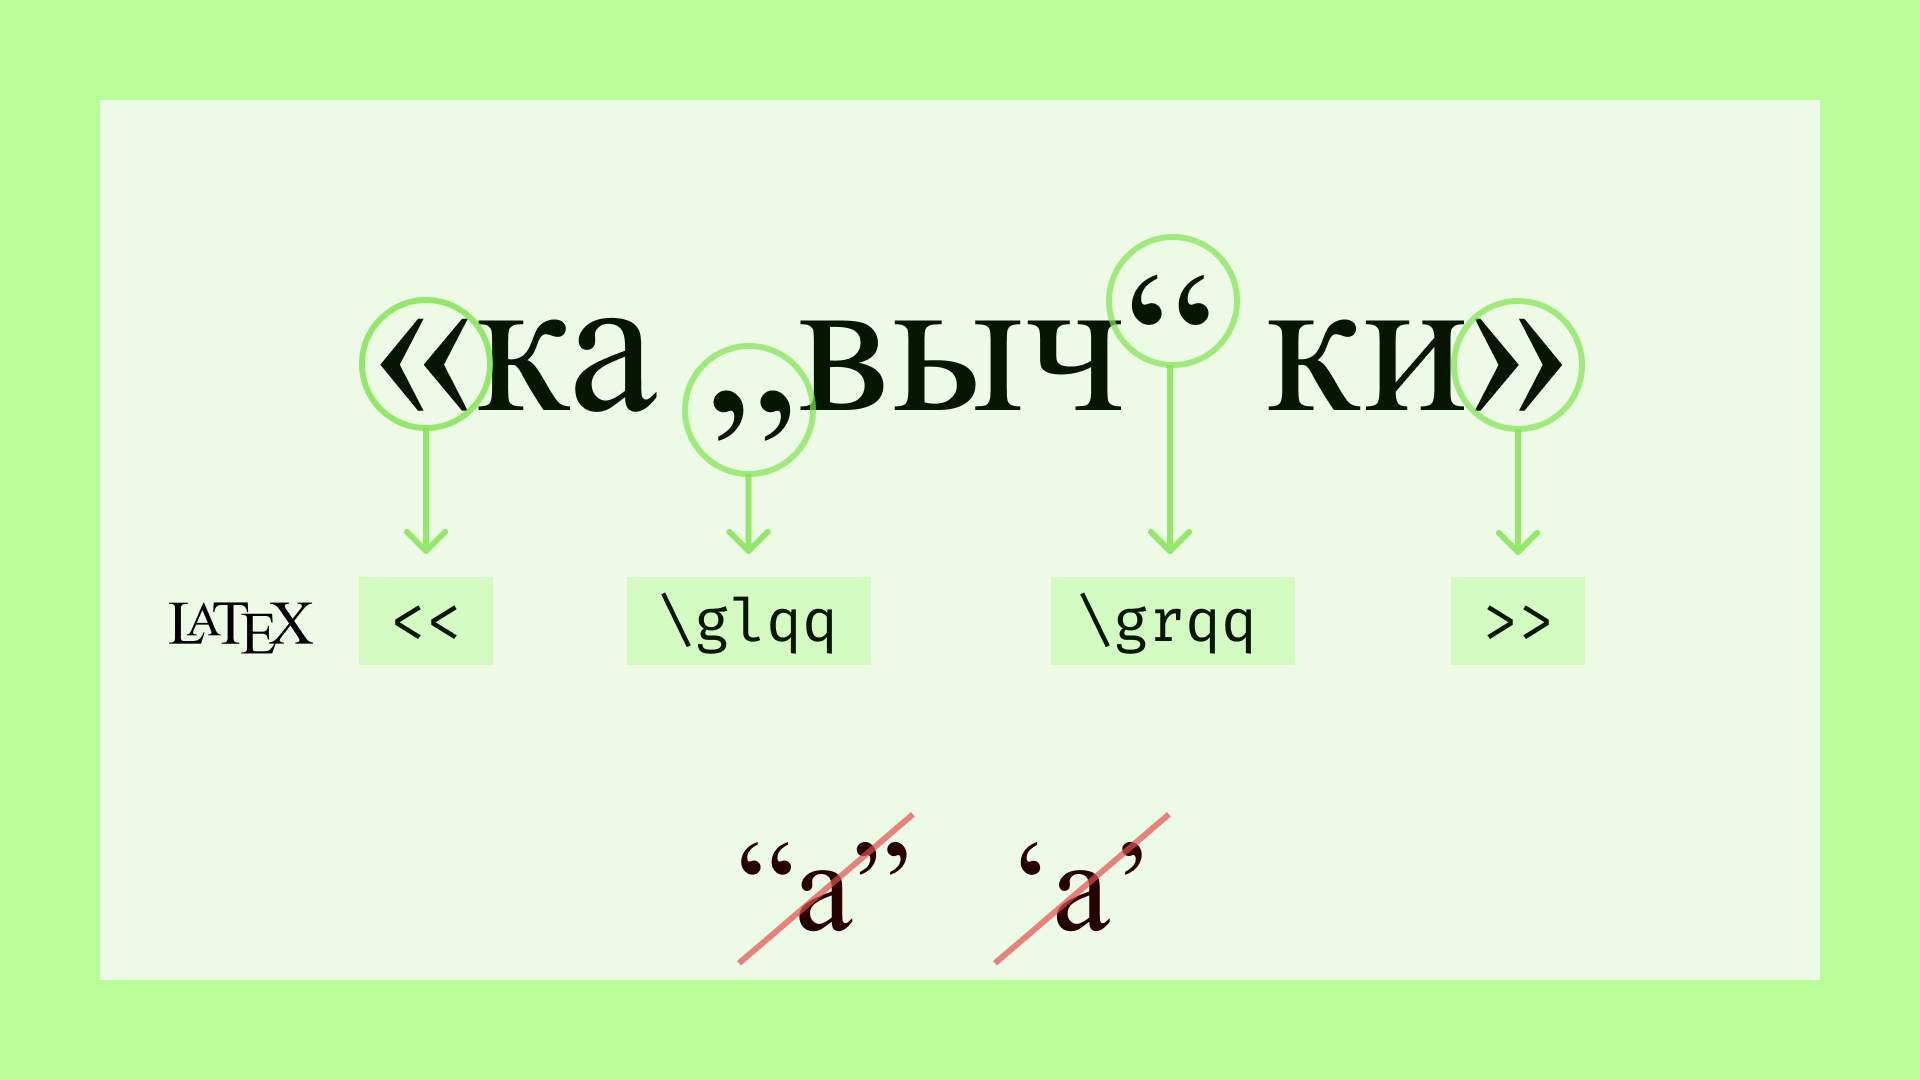
\includegraphics[width=0.9\linewidth]{kavichki.png}
%     \captionsetup{justification=centering, format=plain}
%     \caption{Правильное использование кавычек} % Название рисунка
%     \label{fig:pic21}
% \end{figure}

\myfigure{0.9}{kavichki.png}{Правильное использование кавычек}{pic21}

Вставка нумерованной формулы.
\begin{equation}
P_{gen}=P_{f} + P_S + P_C + P^3 + P_P
\label{eq}
\end{equation}

Вставка формулы в тексте \(P_{gen}=P_{f} + P_S + P_C + P_3 + P_P\). Рекомендуется использовать \verb|\[...\]| для выключенных (на отдельной строке) формул вместо \verb|$$...$$|.  Для встроенных в текст формул использовать  \verb|\(...\)|, а не \verb|$...$|. Ссылка на формулу --- формула (\ref{eq}).

Вставка таблиц

На все таблицы в тексте должны быть ссылки. Таблица должна располагаться непосредственно после текста, в котором она упоминается впервые, или на следующей странице. Пример ссылки на таблицу: Полученные данные занесены в таблицу \ref{table:table21}.

\renewcommand{\arraystretch}{1}  % увеличение высоты ячеек если нужно
\begin{table}[H]
    \centering   % располагаем таблицу по центру
    \caption{Пример названия таблицы}    % название таблицы
    \begin{tabular}{|m{5cm}|m{5cm}|m{5cm}|}        % описываем 3 столбца таблицы
    \hline   % горизонтальная черта
     &  \centering\arraybackslash Заголовок столбца 1 & \centering\arraybackslash Заголовок столбца 2 \\ \hline
    Заголовок строки 1 & Значение & Значение \\ \hline
    Заголовок строки 2 & Значение & Значение \\ \hline
    \end{tabular}
    \label{table:table21}
\end{table}

Вставка длинной таблицы

Лучше избегать вставки длинной таблицы в тексте работы и перенести ее в приложение. 

Если это все-таки необходимо, важно не забывать писать <<Продолжение Таблицы (номер таблицы)>> или <<Окончание таблицы  (номер таблицы)>>, когда она переходит на новую страницу (табл. \ref{longtable:dlin_tabl}). Не нужно проводить черную линию перед переносом таблицы. Как это делать --- смотрите в коде документа. 

Текст в ячейках-заголовках должен быть по центру. Текст остальных ячеек должен быть выравнен по левому краю. Правильное оформление длинной таблицы ниже.

\hfill\break 
\hfill\break 
\hfill\break 
\hfill\break 
\hfill\break 
\hfill\break 
\hfill\break
\hfill\break
(пустое пространство, чтобы показать перенос таблицы)
\hfill\break 
\hfill\break 
\hfill\break 
\hfill\break 
\hfill\break 
\hfill\break 
\hfill\break
\hfill\break

\renewcommand{\arraystretch}{1.1} % увеличение высоты ячеек если нужно
\newcolumntype{J}{ >{\arraybackslash} m{2cm} }
\newcolumntype{B}{ >{\arraybackslash} m{6cm} } % здесь можно указать правило выравнивания и ширину стобца
% Из-за того, что мы прописали \centering в настройках столбцов выше, иногда нам придется использовать "\tabularnewline" вместо "\\"
\begin{longtable}[h!]{|J|B|B|}
    \caption{Название длинной таблицы} \\
    \hline
    \multicolumn{1}{|c|}{№} & \multicolumn{1}{|c|}{Заголовок столбца 1} & \multicolumn{1}{|c|}{Заголовок столбца 2} \tabularnewline
    \hline
    \multicolumn{1}{|c|}{1} & \multicolumn{1}{|c|}{2} &  \multicolumn{1}{|c|}{3} \tabularnewline
    \hline
    \endfirsthead
    \multicolumn{3}{r}{Окончание таблицы \thetable\hspace{-2em} } \tabularnewline  % корректируйте значение в \hspace{}, чтобы выровнять по правому краю

    \hline
     \multicolumn{1}{|c|}{1} &  \multicolumn{1}{|c|}{2} &  \multicolumn{1}{|c|}{3} \tabularnewline 
    \hline
    \endhead

    \multicolumn{3}{l}{} 
    \endfoot

    \hline
    \endlastfoot


1 & Данные & Данные \\ \hline

2 & Данные & Данные \\ \hline

3 & Данные & Данные \\ \hline

4 & Данные & Данные \\ \hline

5 & Данные & Данные \\  % на месте где разрывается таблица линию не проводим

6 & Данные & Данные \\ \hline 

7 & Данные & Данные \label{longtable:dlin_tabl}\\ % label для создания ссылки ref на таблицу в тексте. Должен находиться именно внутри какой-нибудь ячейки, иначе таблица ломается.

\end{longtable}

Листинг кода

Небольшой программный код, который нужно продемонстрировать в работе, можно представить в виде иллюстрации (скриншота) в тексте работы с соблюдением правил оформления для рисунков. В случае длинного листинга рекомендуется располагать его в приложении или иллюстрацией, или текстом. Пример оформления листинга в текстовом виде приведён в приложении Б. Вставка кода из файла продемонстрирована в приложении~В.



\section*{Выводы по главе}
\addcontentsline{toc}{section}{Выводы по главе}
Краткое описание того, что было в главе. Сделайте акцент на том, что было сделано вами лично.

\chapter*{ЗАКЛЮЧЕНИЕ}
\addcontentsline{toc}{chapter}{ЗАКЛЮЧЕНИЕ} % это будет отображаться в содержании

В заключении указывается основной результат работы и побочные результаты, если студент считает это необходимым. Дается оценка полноты решений поставленных задач. Прописывается, что планируется сделать в дальнейшем, если курсовая будет продолжаться в дипломе. 

Курсовая или дипломная работа подается на нормоконтроль за нес\-колько дней до защиты. Нормоконтролеру нужно высылать только pdf-файл, а после получения ответа от нормоконтролера ошибки устраняются, и работа посылается на проверку еще раз, и так до тех пор, пока нормоконтролер не одобрит работу.




\chapter*{СПИСОК ИСПОЛЬЗОВАННЫХ ИСТОЧНИКОВ}
\addcontentsline{toc}{chapter}{СПИСОК ИСПОЛЬЗОВАННЫХ ИСТОЧНИКОВ} % это будет отображаться в содержании
%\renewcommand{\bibsection}{\centering\textbf{\large СПИСОК ИСПОЛЬЗОВАННЫХ ИСТОЧНИКОВ}} % смена названия библиографии по умолчанию
%\bibliographystyle{biblio/gost2008n} % файл, задающий формат ссылок по ГОСТ
%\bibliography{biblio/biblio} % файл с библиографией

\begin{thebibliography}{}

\bibitem{bib_gost1}
    Отчёт о научно-исследовательской работе. Структура и правила оформления. : ГОСТ 7.32--2017 : национальный стандарт : дата введения 2018–07–01
    
\bibitem{bib_gost2} 
    Библиографическая запись. Библиографическое описание. Общие требования и правила составления : ГОСТ Р 7.0.100-–2018 : национальный стандарт : дата введения 2019-07–01
\bibitem{bib_electr_res} 
    Overleaf. Изучите LaTeX за 30 минут : [Электронный ресурс]. --– URL: https://www.overleaf.com/learn/latex/Learn\_LaTeX\_in\_30\_minutes \break(дата обращения: 21.03.2024).

\bibitem{bib_author}
    Вятчина О. Ф. Малый практикум по микробиологии : Учеб.-метод. пособие / О. Ф. Вятчина, Н. Е. Буковская, О. А. Жилкина. –- Иркутск : Изд-во Иркут. гос. ун-та, 2009. –- 129 с. : ил. –- Библиогр.: с. 128–129.

\bibitem{bib_setev_elect_res}
    Об объектах культурного наследия (памятники истории и культуры) народов Российской Федерации в Иркутской области [Электронный ресурс]  : закон Иркут. обл. от 23.07.2008 № 57-оз (в ред. От 05.042010). --– Документ опубликован не был. --– Доступ из справ. Правовой системы «КонсультантПлюс» в локальной сети Науч. б-ки Иркут. гос. ун-та.
    
\bibitem{bib_udal_res_site}
    Аргучинцев А. В. Оптимальное управление начальными условиями канонической гиперболической системы первого порядка на основе нестандартных формул приращения [Электронный ресурс] / А. В. Аргучинцев, В. П. Поплевко // Изв. вузов. Математика. –- 2008. --– № 1. --– С. 3–-10. --– Электрон. Версия печат. \breakПублик. . –- Систем. Требования: Adode Acrobat Reader/ --- URL: http: //ellib.librery.isu.ru/docs/social/p1422\_D19\_7525.pdf/ (дата обращения: 10.08.2010).

\end{thebibliography}


\chapter*{ПРИЛОЖЕНИЯ}
\addcontentsline{toc}{chapter}{ПРИЛОЖЕНИЯ}

%% ДЛЯ ОТЧЕТОВ ПО ПРАКТИКЕ: вставить ежедневные записи студента можно по аналогии с титульном листом, таким образом:
% \newpage     % обязательно для правильной нумерации страниц в Содержании
%% команду chapter не используем, заголовок должен быть прямо в pdf
% \addcontentsline{toc}{chapter}{ПРИЛОЖЕНИЯ}
% \addcontentsline{toc}{section}{Приложение А Ежедневные записи студента по практике}
% \includepdf[pages={1}]{vashi_zapisi_studenta.pdf}     % файл конвертированный из docx с таблицей и всеми заголовками + номер страницы(!)

\begin{flushright}
     \bfПриложение А
\end{flushright}

\begin{center}  \bfНазвание приложения \end{center}
\addcontentsline{toc}{section}{Приложение А Название приложения}

Приложения обозначают заглавными буквами русского алфавита, начиная с А, за исключением букв Ё, З, Й, О, Ч, Ь, Ы, Ъ. После слова «Приложение» следует буква, обозначающая его последовательность.
Если в документе одно приложение, оно обозначается «Приложение А».
Каждое приложение начинается с новой страницы.
{\bf В тексте документа должны быть ссылки на все приложения.}  Приложения располагают в порядке ссылок на них в тексте документа.

Приложения могут включать: графический материал, таблицы, расчеты, описания алгоритмов и программ. Длинные таблицы, большие расчеты, длинные алгоритмы и программы рекомендуется помещать именно в приложения, а не в основной части работы. Здесь можно разместить ссылку на Github со своей работой, если нужно. Например, вот так:

Ссылка на репозиторий проекта: https://github.com/latex3/latex2e

Иллюстрации, таблицы, формулы в пределах каждого приложения обозначают отдельной нумерацией арабскими цифрами с добавлением впереди обозначения приложения (например: Рисунок А.1 или Таблица Б.2, к формуле просто (В.1)).
\newpage

\begin{flushright}
     \bfПриложение Б
\end{flushright}

\begin{center}  \bfПример листинга кода \end{center}
\addcontentsline{toc}{section}{Приложение Б Пример листинга кода}
%% В тексте работы кусочки кода нужно вставлять как рисунок. В приложении можно и так:

%% пропишите нужный вам язык программирования в language 
%% если рамка вокруг листинга вам не нужна - удалите параметр frame
\begin{lstlisting}[language=C, frame=single]  
#include <stdio.h>

int main() {
    int n, i, flag = 0;
    
    printf("Введите положительное целое число: ");
    scanf("%d", &n);
    
    for (i = 2; i <= n / 2; ++i) {
        // Проверка на простое число
        if (n % i == 0) {
            flag = 1;
            break;
        }
    }
    
    if (n == 1) {
        printf("1 не является ни простым, ни составным.\n");
    } else {
        if (flag == 0)
            printf("%d - простое число.\n", n);
        else
            printf("%d - составное число.\n", n);
    }
    
    return 0;
\end{lstlisting}
\newpage


\begin{flushright}
     \bfПриложение В
\end{flushright}

\begin{center}  \bfВторой пример листинга кода \end{center}
\addcontentsline{toc}{section}{Приложение В Второй пример листинга кода}

\lstinputlisting[language=python, frame=single]{Listings/main.py}


\newpage


\begin{flushright}
     \bfПриложение Г
\end{flushright}

\begin{center}  \bfПример вставки рисунка \end{center}
\addcontentsline{toc}{section}{Приложение В Пример вставки рисунка}

В приложении лучше использовать классический способ вставки рисунка, где можно закомментировать подпись и ссылку, так как они нам здесь не нужны.

\begin{figure}[H]
\centering
    % width - отвечает за размер вашего рисунка
    % {kavichki.png} - это название рисунка из папки Images
    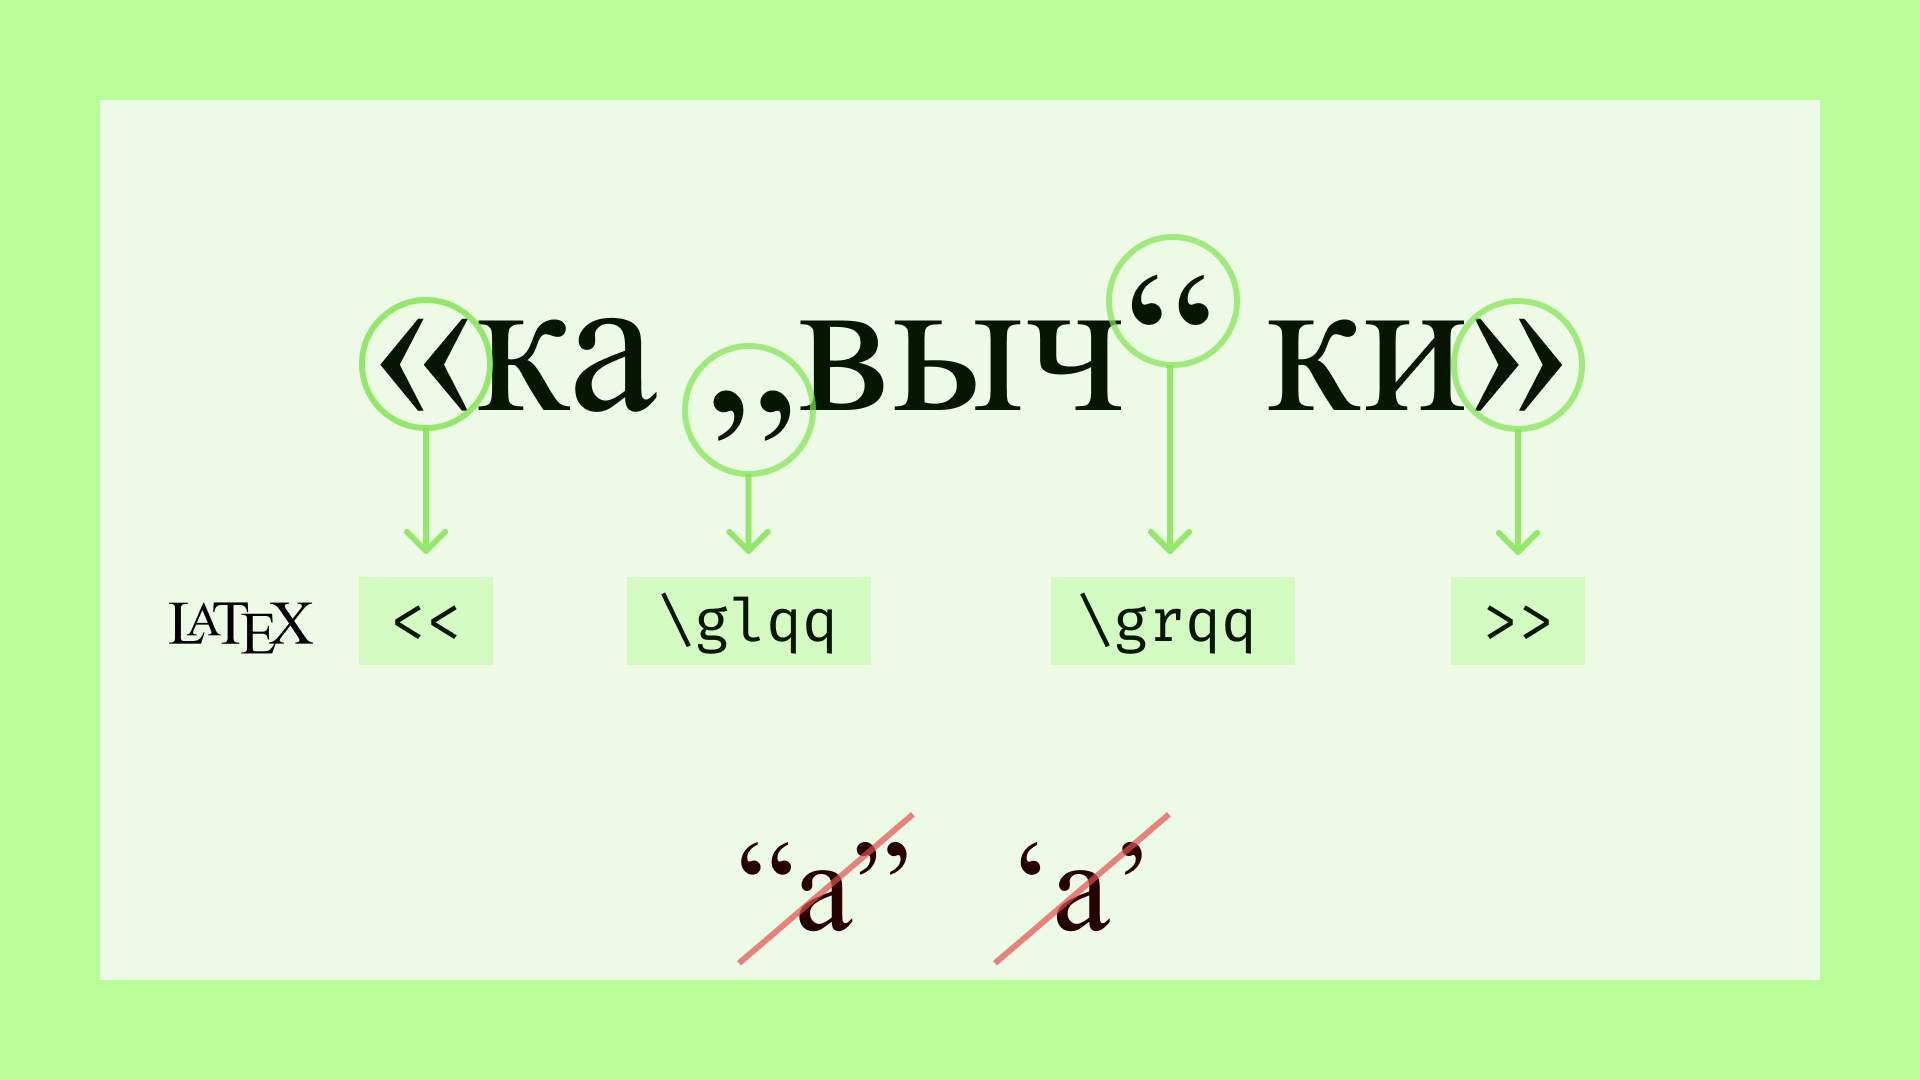
\includegraphics[width=1\linewidth]{kavichki.png}
    \captionsetup{justification=centering, format=plain}
    \caption{Правильное использование кавычек} % Название рисунка
    \label{fig:pic21}
\end{figure}

\end{document}
